\renewcommand{\thesection}{\arabic{section}}\renewcommand{\theHsection}{chapter.\arabic{section}}\setcounter{section}{10}\section{曲线积分}
\noindent\begin{minipage}{\textwidth}\ProblemHeading{例题}{11.1}
计算第一型曲线积分 $\displaystyle\int_\Gamma\frac{z^2}{x^2+y^2}\,ds$，其中 $\Gamma$ 为圆柱螺线 $x=a\cos t,\ y=a\sin t,\ z=bt$（$0\le t\le2\pi$），$a>0$。
\end{minipage}\par\vfill
\noindent\begin{minipage}{\textwidth}\ProblemHeading{例题}{11.2}
设 $a>0$，$\Gamma$ 为球面 $x^2+y^2+z^2=a^2$ 与平面 $x+y+z=0$ 的交圆。计算 $\int_\Gamma xy\,ds$。
\end{minipage}\par\vfill
\noindent\begin{minipage}{\textwidth}\ProblemHeading{习题}{11.3}
计算下列第一型曲线积分，其中 $a>0$。
\SubQ{1}{$\displaystyle\int_\Gamma(x^2+y^2)^n\,ds$，$\Gamma:x=a\cos t,\ y=a\sin t$（$0\le t\le2\pi$），$n\in\mathbb N^*$。}
\SubQ{2}{$\displaystyle\int_\Gamma(x+y)\,ds$，$\Gamma$ 为顶点 $(0,0),(1,0),(0,1)$ 的三角形边界。}
\SubQ{3}{$\displaystyle\int_\Gamma z\,ds$，$\Gamma:x=t\cos t,\ y=t\sin t,\ z=t$（$0\le t\le2\pi$）。}
\end{minipage}\par\vfill
\newpage
\noindent\begin{minipage}{\textwidth}\ProblemHeading{习题}{11.4}
计算下列第一型曲线积分，其中 $a>0$。
\SubQ{1}{$\displaystyle\int_\Gamma x^2\,ds$，$\Gamma$ 为圆周 $x^2+y^2+z^2=a^2,\ x+y+z=0$。}
\SubQ{2}{$\displaystyle\int_\Gamma y^2\,ds$，$\Gamma$ 为旋轮线的一拱：$x=a(t-\sin t),\ y=a(1-\cos t)$（$0\le t\le2\pi$）。}
\end{minipage}\par\vfill
\noindent\begin{minipage}{\textwidth}\ProblemHeading{例题}{11.5}
计算第二型曲线积分 $\int_Kxy\,dx$、$\int_Lxy\,dx$、$\int_Mxy\,dx$。其中 $K$ 为从 $(0,0)$ 到 $(1,1)$ 的直线段；$L$ 为抛物线 $y=x^2$ 从 $(0,0)$ 到 $(1,1)$ 的一段；$M$ 为依次经过 $(0,0),(1,0),(1,1)$ 的有向折线。
\end{minipage}\par\vfill
\noindent\begin{minipage}{\textwidth}\ProblemHeading{例题}{11.6}
设 $a>0$，$\Gamma$ 为球面 $x^2+y^2+z^2=a^2$ 与平面 $x+y+z=0$ 的交圆，从第一卦限看其方向为逆时针。计算 $\int_\Gamma x\,dx+y\,dy+z\,dz$。
\end{minipage}\par\vfill
\newpage
\noindent\begin{minipage}{\textwidth}\ProblemHeading{习题}{11.7}
计算下列第二型曲线积分，其中 $a,b>0$。
\SubQ{1}{$\displaystyle\int_\Gamma\frac{x\,dy-y\,dx}{x^2+y^2}$，$\Gamma$ 为逆时针圆周 $x^2+y^2=a^2$。}
\SubQ{2}{$\displaystyle\int_\Gamma(x+y)\,dx+(x-y)\,dy$，$\Gamma$ 为逆时针椭圆 $x^2/a^2+y^2/b^2=1$。}
\SubQ{3}{$\displaystyle\int_\Gamma(x^2-2xy)\,dx+(y^2-2xy)\,dy$，$\Gamma:x=y^2$（$-1\le y\le1$），沿 $y$ 增加的方向。}
\end{minipage}\par\vfill
\noindent\begin{minipage}{\textwidth}\ProblemHeading{习题}{11.8}
计算下列第二型曲线积分，其中 $a,b>0$。
\SubQ{1}{$\displaystyle\int_\Gamma x\,dy$，$\Gamma$ 为直线 $2x+y=1$ 与两坐标轴围成的三角形边界，沿逆时针方向。}
\SubQ{2}{$\displaystyle\int_\Gamma(x^2+y^2)\,dy$，$\Gamma$ 为 $x=1,x=3,y=1,y=4$ 所围矩形的边界，沿逆时针方向。}
\end{minipage}\par\vfill
\noindent\begin{minipage}{\textwidth}\ProblemHeading{习题}{11.9}
设常数 $a,b,c$ 满足 $ac-b^2>0$，$\Gamma$ 为逆时针单位圆周。计算 $\displaystyle\int_\Gamma\frac{x\,dy-y\,dx}{ax^2+2bxy+cy^2}$。
\end{minipage}\par\vfill
\newpage
\noindent\begin{minipage}{\textwidth}\ProblemHeading{习题}{11.10}
计算下列第二型曲线积分，曲线正向为参数增加的方向。
\SubQ{1}{$\displaystyle\int_\Gamma xz^2\,dx+yx^2\,dy+zy^2\,dz$，$\Gamma:x=t,\ y=t^2,\ z=t^3$（$0\le t\le1$）。}
\SubQ{2}{$\displaystyle\int_\Gamma(y+z)\,dx+(z+x)\,dy+(x+y)\,dz$，$\Gamma:x=a\sin^2t,\ y=2a\sin t\cos t,\ z=a\cos^2t$（$0\le t\le\pi$），$a>0$。}
\end{minipage}\par\vfill
\noindent\begin{minipage}{\textwidth}\ProblemHeading{习题}{11.11}
计算 $\displaystyle\int_\Gamma(y^2-z^2)\,dx+(z^2-x^2)\,dy+(x^2-y^2)\,dz$，其中 $\Gamma$ 为球面片 $x^2+y^2+z^2=1,\ x,y,z\ge0$ 的边界，方向为 $(1,0,0)\to(0,1,0)\to(0,0,1)\to(1,0,0)$。
\end{minipage}\par\vfill
\noindent\begin{minipage}{\textwidth}\ProblemHeading{习题}{11.12}
设 $\Gamma$ 为分段光滑有向曲线，$F$ 为其上的连续向量场。证明 $\displaystyle\left|\int_\Gamma F\cdot d\mathbf p\right|\le\int_\Gamma\|F\|\,ds$。
\end{minipage}\par\vfill
\newpage
\noindent\begin{minipage}{\textwidth}\ProblemHeading{例题}{11.13（改写）}
设平面闭区域 $D$ 适用 Green 公式，$\partial D$ 取使区域位于左侧的正向。证明其面积满足\[\sigma(D)=\int_{\partial D}x\,dy=-\int_{\partial D}y\,dx=\frac12\int_{\partial D}(x\,dy-y\,dx).\]
\end{minipage}\par\vfill
\noindent\begin{minipage}{\textwidth}\ProblemHeading{例题}{11.14}
设 $a,b>0$。利用 Green 公式计算椭圆 $x^2/a^2+y^2/b^2=1$ 所围图形的面积。
\end{minipage}\par\vfill
\noindent\begin{minipage}{\textwidth}\ProblemHeading{例题}{11.15（改写）}
设 $\Gamma$ 为逆时针单位圆周。计算 $\displaystyle\int_\Gamma\frac{x\,dy-y\,dx}{x^2+y^2}$，并说明为何不能直接在单位圆盘上套用 Green 公式。
\end{minipage}\par\vfill
\newpage
\noindent\begin{minipage}{\textwidth}\ProblemHeading{例题}{11.16（校订）}
设 $\Gamma$ 为包围原点且不经过原点的分段光滑简单闭曲线，沿逆时针方向。计算 $\displaystyle\int_\Gamma\frac{x\,dy-y\,dx}{x^2+y^2}$。
\end{minipage}\par\vfill
\noindent\begin{minipage}{\textwidth}\ProblemHeading{例题}{11.17（改写）}
判断图中所示的四个平面区域分别是单连通还是多连通，并说明理由。这里若区域内的每条简单闭曲线所围成的有界区域都包含在原区域内，就称原区域单连通。
\begin{center}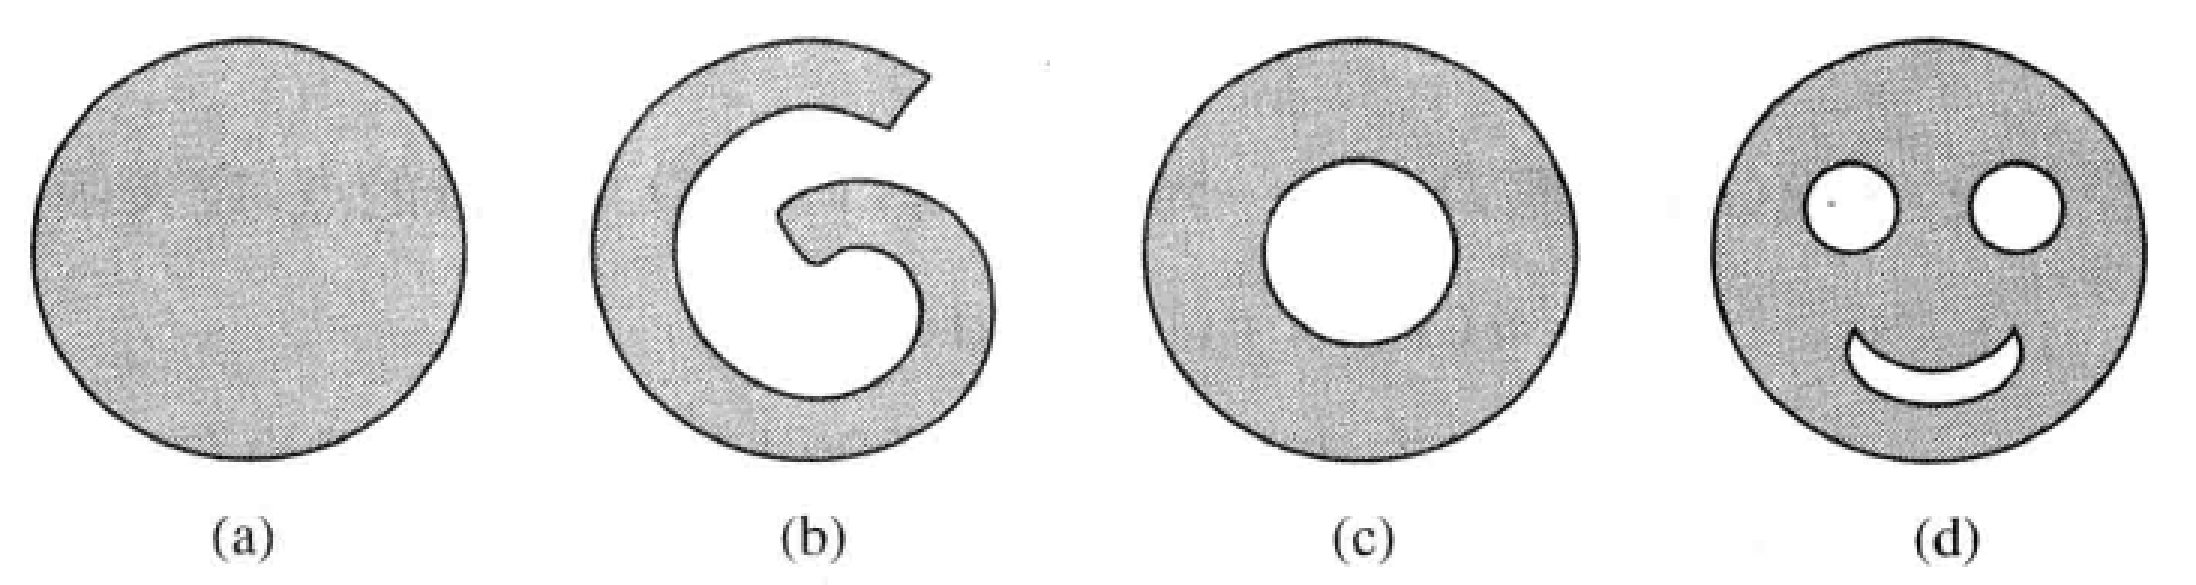
\includegraphics[width=0.85\linewidth]{figures/fig_11_17_1.png}\end{center}
\end{minipage}\par\vfill
\noindent\begin{minipage}{\textwidth}\ProblemHeading{例题}{11.18}
计算曲线积分 $\displaystyle\int_L\frac{x\,dy-y\,dx}{(x-y)^2}$，其中 $L$ 为从 $A=(0,-1)$ 到 $B=(1,0)$ 且不经过直线 $y=x$ 的任意分段光滑路径。
\end{minipage}\par\vfill
\newpage
\noindent\begin{minipage}{\textwidth}\ProblemHeading{习题}{11.19}
利用 Green 公式计算下列积分，其中 $a,b>0$。
\SubQ{1}{$\displaystyle\int_\Gamma xy^2\,dy-x^2y\,dx$，$\Gamma$ 为逆时针圆周 $x^2+y^2=a^2$。}
\SubQ{2}{$\displaystyle\int_\Gamma(x+y)\,dx-(x-y)\,dy$，$\Gamma$ 为逆时针椭圆 $x^2/a^2+y^2/b^2=1$。}
\SubQ{3}{$\displaystyle\int_\Gamma e^x\sin y\,dx+e^x\cos y\,dy$，$\Gamma$ 为上半圆周 $x^2+y^2=ax$（$y\ge0$），沿 $x$ 增加的方向。}
\end{minipage}\par\vfill
\noindent\begin{minipage}{\textwidth}\ProblemHeading{习题}{11.20}
利用 Green 公式计算下列曲线所围图形的面积，其中 $a>0$。
\SubQ{1}{星形线 $x=a\cos^3t,\ y=a\sin^3t$（$0\le t\le2\pi$）。}
\SubQ{2}{双纽线 $(x^2+y^2)^2=a^2(x^2-y^2)$。}
\SubQ{3}{Descartes 叶形线 $x^3+y^3=3axy$ 的闭环。}
\end{minipage}\par\vfill
\noindent\begin{minipage}{\textwidth}\ProblemHeading{习题}{11.21}
设分段光滑简单闭曲线 $\Gamma$ 由 $x=\varphi(t),\ y=\psi(t)$（$\alpha\le t\le\beta$）参数化，参数增加时沿正向。证明其所围区域面积为\[A=\frac12\int_\alpha^\beta\begin{vmatrix}\varphi(t)&\psi(t)\\\varphi^{\prime}(t)&\psi^{\prime}(t)\end{vmatrix}dt.\]
\end{minipage}\par\vfill
\newpage
\noindent\begin{minipage}{\textwidth}\ProblemHeading{习题}{11.22}
设单变量函数 $f$ 连续可微，$\Gamma$ 为任意分段光滑闭曲线。证明：
\SubQ{1}{$\displaystyle\int_\Gamma f(xy)(y\,dx+x\,dy)=0$。}
\SubQ{2}{$\displaystyle\int_\Gamma f(x^2+y^2)(x\,dx+y\,dy)=0$。}
\SubQ{3}{$\displaystyle\int_\Gamma f(x^n+y^n)(x^{n-1}\,dx+y^{n-1}\,dy)=0$，$n\in\mathbb N^*$。}
\end{minipage}\par\vfill
\noindent\begin{minipage}{\textwidth}\ProblemHeading{习题}{11.23}
设 $\Gamma$ 为平面光滑简单闭曲线，$\mathbf n$ 为其单位外法向量，$\mathbf a$ 为固定单位向量。证明 $\int_\Gamma\cos\angle(\mathbf a,\mathbf n)\,ds=0$。
\end{minipage}\par\vfill
\noindent\begin{minipage}{\textwidth}\ProblemHeading{习题}{11.24}
设 $\Gamma$ 为平面光滑简单闭曲线，$\mathbf n$ 为单位外法向量，$\mathbf i,\mathbf j$ 为坐标单位向量。用所围区域的面积表示曲线积分\[\int_\Gamma\bigl(x\cos\angle(\mathbf n,\mathbf i)+y\cos\angle(\mathbf n,\mathbf j)\bigr)\,ds.\]
\end{minipage}\par\vfill
\newpage
\noindent\begin{minipage}{\textwidth}\ProblemHeading{习题}{11.25（校订）}
计算下列曲线积分。
\SubQ{1}{$\displaystyle\int_L(x^2+2xy-y^2)\,dx+(x^2-2xy-y^2)\,dy$，$L$ 为从 $(0,0)$ 到 $(2,1)$ 的任意光滑曲线段。}
\SubQ{2}{$\displaystyle\int_L\frac{(x+y)\,dx-(x-y)\,dy}{x^2+y^2}$，$L$ 为从 $(-1,0)$ 到 $(1,0)$ 的任意光滑曲线，其余点均在上半平面 $y>0$。}
\end{minipage}\par\vfill
\noindent\begin{minipage}{\textwidth}\ProblemHeading{习题}{11.26（校订）}
设 $\Gamma$ 为原点在其内部、沿逆时针方向的分段光滑简单闭曲线。计算\[\int_\Gamma\frac{e^x}{x^2+y^2}\bigl((x\sin y-y\cos y)\,dx+(x\cos y+y\sin y)\,dy\bigr).\]
\end{minipage}\par\vfill
\noindent\begin{minipage}{\textwidth}\ProblemHeading{习题}{11.27}
设 $P,Q$ 在 $\mathbb R^2$ 上具有连续偏导数。对任意中心 $(x_0,y_0)$ 和任意半径 $r>0$，以 $\Gamma$ 表示相应上半圆周。若 $\int_\Gamma P(x,y)\,dx+Q(x,y)\,dy=0$ 恒成立，证明在 $\mathbb R^2$ 上 $P=0$ 且 $\partial Q/\partial x=0$。
\end{minipage}\par\vfill
\newpage
\noindent\begin{minipage}{\textwidth}\ProblemHeading{习题}{11.28}
设 $\Gamma$ 为平面光滑简单闭曲线，围成区域 $G$，$u,v$ 在 $\overline G$ 的邻域内为 $C^2$ 函数，$\partial/\partial n$ 表示沿单位外法向量的导数，$\Delta=\partial_x^2+\partial_y^2$。证明 Green 第二公式\[\iint_G\begin{vmatrix}\Delta u&\Delta v\\u&v\end{vmatrix}dx\,dy=\int_\Gamma\begin{vmatrix}\partial u/\partial n&\partial v/\partial n\\u&v\end{vmatrix}ds.\]
\end{minipage}\par\vfill
\noindent\begin{minipage}{\textwidth}\ProblemHeading{习题}{11.29}
设平面光滑简单闭曲线 $\Gamma$ 围成区域 $G$，$u$ 在 $\overline G$ 的邻域内调和，即 $\Delta u=0$。对 $(x_0,y_0)\in G$，记 $r=\sqrt{(x-x_0)^2+(y-y_0)^2}$，$\partial/\partial n$ 为外法向导数。证明\[u(x_0,y_0)=\frac1{2\pi}\int_\Gamma\left(u\frac{\partial\ln r}{\partial n}-\ln r\frac{\partial u}{\partial n}\right)ds.\]
\end{minipage}\par\vfill
\noindent\begin{minipage}{\textwidth}\ProblemHeading{习题}{11.30（校订）}
设 $G\subset\mathbb R^2$ 为区域，$u$ 在 $G$ 内调和。设以 $(x_0,y_0)$ 为中心、半径 $R>0$ 的闭圆盘包含于 $G$，其边界为 $\Gamma$。证明\[u(x_0,y_0)=\frac1{2\pi R}\int_\Gamma u(x,y)\,ds.\]
\end{minipage}\par\vfill
\newpage
\noindent\begin{minipage}{\textwidth}\ProblemHeading{例题}{11.31（改写）}
判断下列推理是否正确，并说明理由：“对任意大于 $1$ 的正整数 $n$，有 $n^2>n$，所以 $n$ 不可能是最大的正整数；于是 $1$ 就是最大的正整数。”讨论这一推理与最大值存在性之间的关系。
\end{minipage}\par\vfill
\noindent\begin{minipage}{\textwidth}\ProblemHeading{习题}{11.32}
设平面分段光滑简单闭曲线 $\Gamma$ 的周长为 $L$，所围区域面积为 $A$。证明 $A\le L^2/(4\pi)$，且等号当且仅当 $\Gamma$ 为圆周时成立。
\end{minipage}\par\vfill
\noindent\begin{minipage}{\textwidth}\ProblemHeading{习题}{11.33}
证明：周长为 $L$ 的四边形中，正方形的面积最大。
\end{minipage}\par\vfill
